\chapter{Háttérismeretek}

\section{Kapocsolódó munkák}
%TODO: 

\section{SysML}

A System Modeling Language (SysML) egy általános célú architektúra modellező nyelv, melyet elsősorban rendszermérnökök használnak. A nyelvvel különböző komplex rendszereket tudunk leírni többféle megközelítésből mint magas szintű funkcionális modellek mind pedig az alacsonyabb akár fizikai modellekig.

A SysML-t mint ahogyan az UML-t is az Object Management Group (OMG) fejleszti, sőt az UML 2-nek egy dialógusa a nyelv, úgynevezett UML profil segítségével van definiálva. Az UML profil a nyelv specializálásának egy módja sztereotípiák (Stereotype), megkötések (Constraint) és címkézett értékek (Tagged Value) segítségével (\refstruc{fig:custom-profile}).

\begin{figure}[!ht]
	\centering
	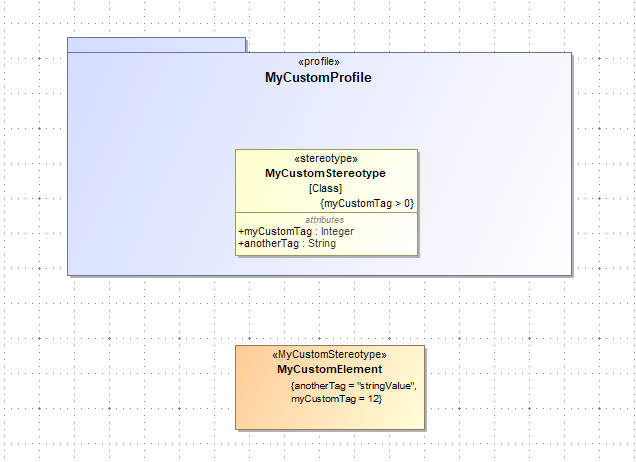
\includegraphics[width=150mm, keepaspectratio]{figures/preliminaries/custom-profile.png}
	\caption{UML nyelv specializálása sztereotípiákkal}
	\label{fig:custom-profile}
\end{figure}

Egy nyelv lehetséges elemeit és kapcsolatait leíró struktúrát metamodellnek hívjuk, a tényleges elemekből és ezek kapcsolatából álló modellt pedig példánymodellnek.  SysML esetében az UML profil az amit metamodellnek tudunk tekinteni, igaz a metaszintek eléggé összemosódnak és nem elegendő csak a profilt ismerni, hanem az UML metamodellt is ismerni kell. Például egy SysML Block valójában egy sztereotipizált UML Class. Ez azt jelenti, hogy van egy UML példány specifikáció (Instance Specification) aminek az osztája (Classifier) egy Block sztereotípia és ez hozzá van rendelve az UML-s osztály példányunkhoz a modellünkben. Az UML-s osztály példány a sztereotípia és a példány specifikáció tehát hagyományos értelemben azonos metaszinten helyezkednek el (\refstruc{fig:block-stereotype}).

\begin{figure}[!ht]
	\centering
	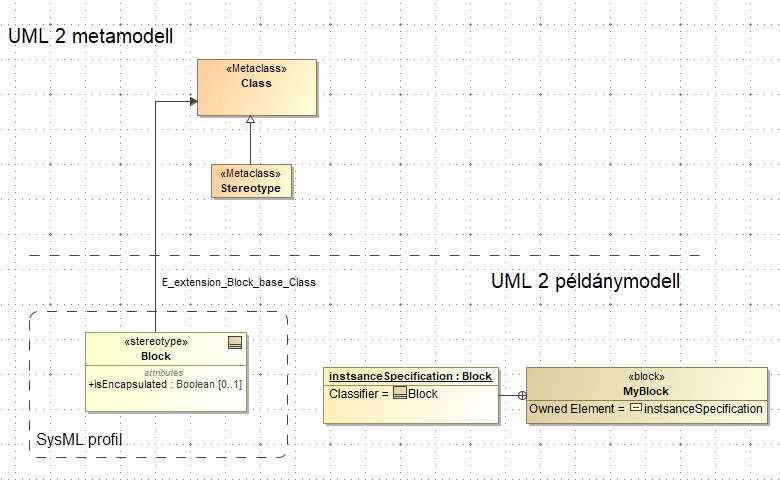
\includegraphics[width=150mm, keepaspectratio]{figures/preliminaries/block-stereotype.png}
	\caption{Meta szintek és Block sztereotípia alkalmazása}
	\label{fig:block-stereotype}
\end{figure}

SysML segítségével sokféle modellt lehet készíteni a teljesség igénye nélkül: Követelmény modellek, viselkedés modellek, struktúra modellek, allokáció modellek, mindezek közül azonban kettőre koncentrálok a dolgozat elkészítése közben, mégpedig a viselkedés modellek egy részére az állapotgépekre és a funkcionális architektúrára amely funkcionális architektúra egy de-komponált állapotgépet ír le.



\subsection{Állapotgépek, állapottérképek}

Állapotgépek (State Machine) alatt olyan modelleket értünk amik a rendszert véges számú jól elkülönülő állapotát írják le, illetve az ezek közötti átmeneteket. Az állapotgépeket SysML-ben állapottérkép diagramokon (Statechart Diagram) tudunk definiálni. Szintaktikáját tekintve oválisok amik állapotokat jelentenek illetve az ezeket összekötő nyilak, melyek az állapotok közötti lehetséges váltások. A nyilak általában címkézettek. A címke három részből állhat: esemény (trigger), őrfeltétel (guard), akció (action).

\lstset{framesep=10pt}
\begin{lstlisting}
	esemény [örfeltétel] / akció
\end{lstlisting}
Állapotváltás egy esemény bekövetkezésekor lehetséges. Amennyiben van őrfeltétel annak igaznak kell lennie. Az állapotváltás bekövetkezését szokás tüzelésnek is nevezni. Ha egy állapotátmenet tüzel és van akció az átmenethez rendelve ez végrehajtódik.
Akció nem csak állapotátmenetek, hanem állapotok be és kilépésénél is végrehajthatók, illetve létezik olyan akció is ami folyamatosan fut amíg a rendszer adott állapotban van.

\begin{figure}[!ht]
	\centering
	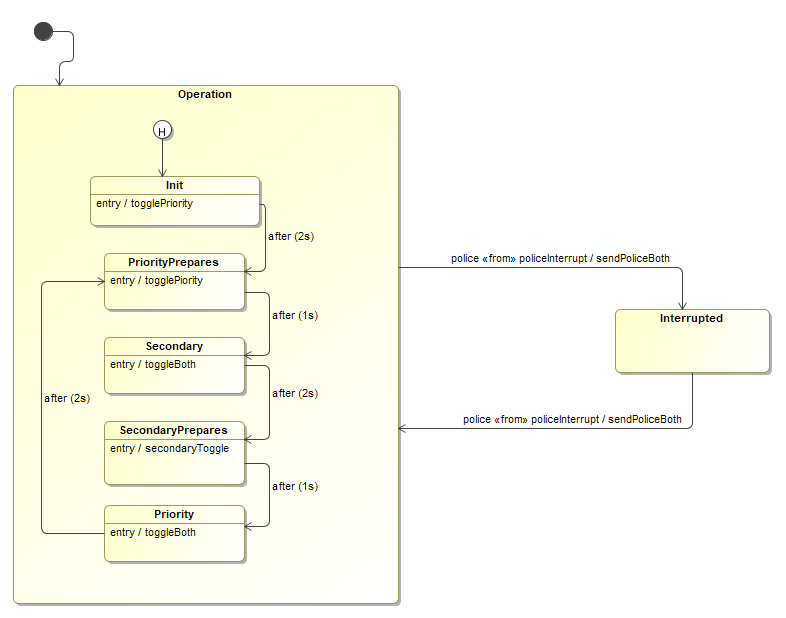
\includegraphics[width=90mm, keepaspectratio]{figures/preliminaries/statechart.png}
	\caption{Állapottérkép SysML-ben}
	\label{fig:statechart}
\end{figure}

Az állapotoknak van egy típusa melyet pszeudo állapotoknak nevezünk. Ezek nem tényleges állapotai a rendszernek olyan értelemben, hogy a rendszer soha nem tartózkodhat ezekben mindig azonnal át kell lépniük belőle egy tényleges állapotba, viszont fontos szemantikai jelentéssel bírnak. A kezdő állapot mely fekete körként jelenik meg egy régió belépési pontjai. Az állapotok mindig régiókban helyezkednek el, ezek tulajdonképpen állapotoknak egy olyan halmaza, amely halmazon belül mindig csak egy állapot lehet aktív, régiókból viszont lehet több is párhuzamosan. Így egy rendszernek lehet egyszerre több aktív állapota is régiónként viszont csak egy (a fork-joinra a dolgozat nem tér ki).

Pszeudo állapotok még a \emph{History Statek} is. Ezek segítségével meg lehet jegyezni, hogy egy összetett állapot mely belső állapota volt aktív, így az állapotba visszalépve nem a belső régió kezdő állapota hanem az utolsó aktív állapot lesz újra aktív. \emph{History State}eknek két változata van \emph{Deep} és \emph{Shallow}. Előbbi egymásba ágyazott esetén minden régióba az utolsó aktív állapotba lép át, míg utóbbi csak a saját régiójának utolsó aktív állapotába. Jelölésük kör benne "H"-val vagy "H*".


\subsection{Funkcionális architektúra modellek}

Egy rendszer funkcionális architektúráján olyan modelleket értünk melyek ennek logikai felépítését írják le azaz, hogy milyen funkciói vannak a rendszernek, ezek hogyan kapcsolódnak egymáshoz. Jelen esetben ezeket a modelleket a rendszer állapotgépének a dekomponálására használjuk. Tehát van egy összetett rendszerünk melyeket funkcionális egységekre tudunk bontani úgy, hogy minden funkcionális egység állapot alapú viselkedések egy összessége. A komponensek képesek egymással kommunikálni és egymás viselkedését ezáltal befolyásolni.

%TODO ez igy meg lehet pontatlan
A rendszert két szempont szerint tudjuk modellezni: komponens definíciók és ezek kompozíciója illetve ezek kapcsolatai szerint. Előbbiek blokkok formájában jelennek meg és SysMLben Blokk definíciós (Block Definition) vagy BDD diagramokon jelennek meg. Azt, hogy a blokkon belüli részek (Part) hogyan kapcsolódnak egymáshoz Internal Block Diagramok (IBD) tartalmazzák. A részek közötti kapcsolatot konnektorok írják le. Ezek jellemzően portokon keresztül kötik össze a részeket. A portok tekinthetők egy adott blokk interfészének is.

A dolgozat elkészítésénél kétféle blokkot különböztetek meg. Azokat melyek állapotgépeket definiálnak és nem bonthatók részekre ezeket állapot blokkoknak nevezem. Illetve olyan blokkokat melyen részekre bonthatók, de nem definiálhatnak saját állapotgépet, ezeket pedig kompozit blokkoknak.

\section{MagicDraw}

A MagicDraw egy modellező eszköz melyet a NoMagic fejlesztett elsősorban UML modellek készítésére. Ahhoz, hogy SyML-ben is tudjunk modelleket készíteni egy beépülő modulra van szükségünk (kivéve ha Cameo System Modellert használunk ami a SysML pluginnal integrálva szállít). A MagicDraw az iparban egy egyre inkább elterjedt eszköz. Szigorúan követi az UML és SysML szabványt.
Az modellezőeszköz gazdag funkcionalitással rendelkezik mint fejlett felhasználói interfész (\refstruc{fig:md-gui}), validációs motor - ami képes akár futásidőben a felhasználók által készített szabályok futtatására is, sablon alapú kódgenerátor és még sok egyéb. Ezen felül a funkcionalitás beépülő modulok segítségével bővíthető.

\begin{figure}[!ht]
	\centering
	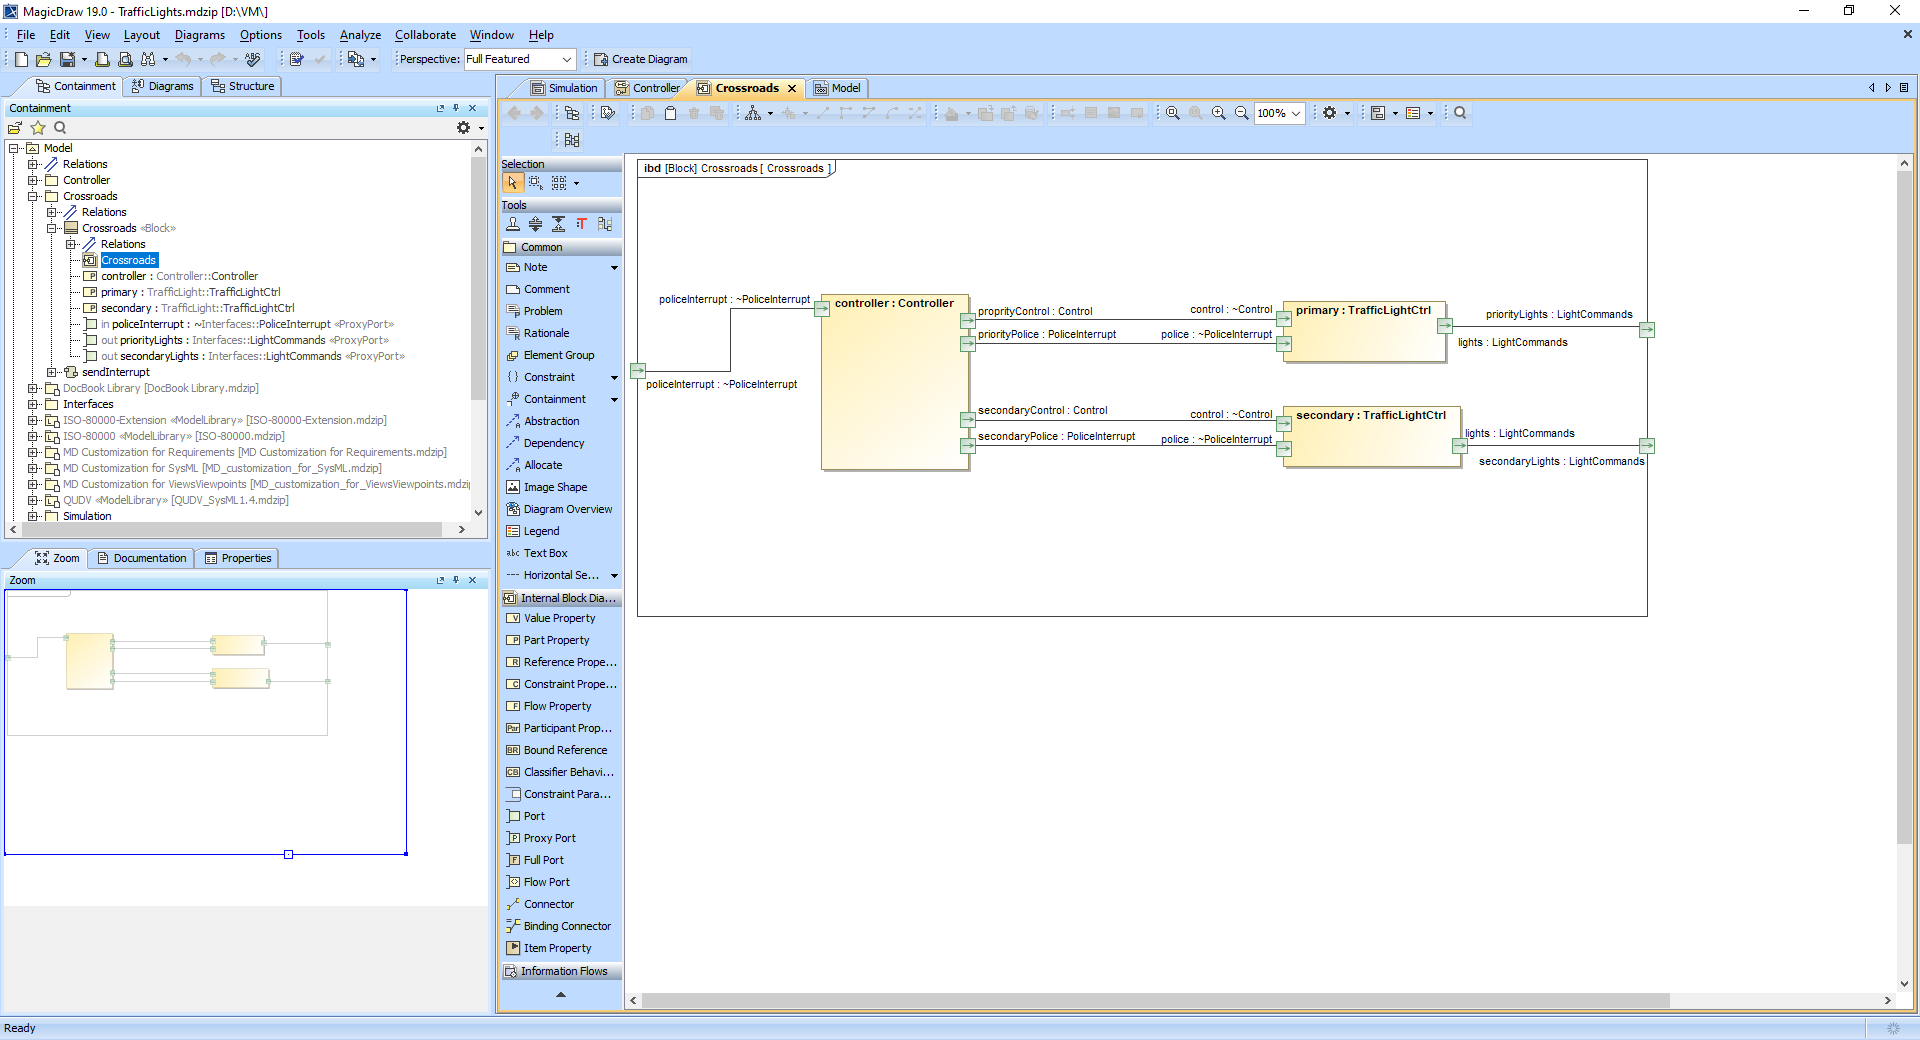
\includegraphics[width=140mm, keepaspectratio]{figures/preliminaries/md-gui.png}
	\caption{MagicDraw felhasználói felülete}
	\label{fig:md-gui}
\end{figure}

MagicDrawhoz lehetőségünk van saját plugin fejlesztésére is, amik lehetővé teszik számunkra, új funkcionalitás integrálását az eszközben illetve modellek manipulálását is. A feladatot is egy ilyen plugin fejlesztésével oldottam meg.


\section{Modelltranszformációk}

Az ipari standardok mellett sok speciális modellezési nyelv is létezik, amelyek megannyi céllal és eszközkészlettel jöttek létre. Ezek között vannak magas absztrakciójú általánosabb nyelvek és alacsony szintűek is amik egy része olyan formalizmusokra épül amik felett bizonyos problémákra matematikai eszközökkel tudunk megoldást keresni.

A modellvezéreltség egyik alapötlete, hogy különböző modellekből származtatni tudunk más modelleket feltéve, hogy elegendő információ áll rendelkezésünkre a konverzió elvégzéséhez. Ezt a fajta származtatást például modell transzformációk segítségével tudjuk végrehajtani. A modelltranszformációk használata lehetővé teszi, hogy ne csak azokat a technológiákat használjuk modellünk feldolgozására melyek speciálisan az adott modellezési nyelvhez készültek hanem a modelleket megpróbáljuk átalakítani - lehetőleg a szemantikai tartalom megőrzésével és automatizáltan - egy olyan modellezési nyelvre amelyhez már létezik az általunk használni kívánt funkcionalitást támogató technológia.

Ezen felül dokumentumokat is tudunk származtatni a modellekből a kódgenerálás tulajdonképpen ennek egy speciális esete. Az sem ritka, hogy a származtatások több lépésen és modellen keresztül történnek. A kód generálásnál maradva a generált kód is egy modell amit általában egy fordítónak valamilyen futtatható állománnyá kell alakítani.


\section{Felhasznált technológiák}

\subsection[]{VIATRA\footnotemark}
\footnotetext{https://www.eclipse.org/viatra/}

A VIATRA egy keretrendszer mely lehetővé teszi eseményvezért modell transzformációk fejlesztését. Ehhez egy inkrementális modell lekérdezéseket leíró nyelvre a VIATRA Query Language-re (\refstruc{fig:vql}) támaszkodik. A létrehozott transzformációkat egy reaktív Query Engine futtatja és tartja karban.

\begin{figure}[!ht]
	\begin{lstlisting}
	pattern StateMachines(stateMachine: StateMachine, name: java String){
	    StateMachine.name(stateMachine, name);
	}
	
	pattern ParametersInStateMachine(stateMachine: StateMachine, parameter: Parameter){
    	StateMachine.ownedParameter(stateMachine, parameter);
	}
	
	pattern RegionsInRegion(container: Region, region: Region){
	    Region.subvertex(container, vertex);
    	State.region(vertex, region);
	}
	\end{lstlisting}
	\caption{Példa: VIATRA Query Language}
	\label{fig:vql}
\end{figure}


A VIATRA használata jelentősen megkönnyíti a modellekkel való munkát, bár én elsősorban a modell lekérdezés részére támaszkodtam a dolgozat elkészítése alatt. MagicDraw-ban egy pluginon keresztül van lehetőség VIATRA használatára melyet V4MD-nek hívnak. A plugin egy Query Engine-t biztosít számunkra per projekt. Ezen keresztül tudunk lekérdezéseket és transzformációkat regisztrálni. A V4MD leveszi a vállunkról a terhet az engine életciklus menedzsmentjét illetően. A VIATRA hátránya lehet azonban, hogy nagyon nagy modelleket komplex lekérdezések esetén a memóriaigénye elég jelentősre duzzadhat a háttérben, cserébe viszont az inkrementális működésnek köszönhetően a lekérdezések már csak a VIATRA által karbantartott táblázatokból való kiolvasás ezért költségül elhanyagolható. Éppen ezért olyan esetekben érdemes használni, amelyek kellően gyakran futnak és gyorsan van szükség az eredmény meghatározására mint például a futás idejű validáció.

\section{MagicDraw állapottérkép verifikációs plugin}

Ebben az alfejezetben bemutatom azt a SysML állapottrékép verifikációs eszközt, mely korábbi egyetemi munkám eredményeként képes volt MagicDraw modellek ellenőrzésére. A funkció megvalósításához a \emph{Gamma Statechart Composition framework} nevű keretrendszert használtam fel.

\subsection{Gamma Statechart Composition Framework}

A Gamma Statechart Composition Framework (továbbiakban Gamma) egy állapottérkép modellező keretrendszer Eclipse felett ami integrálja a YAKINDU-t, de ezen felül saját nyelveket definiál nem csak állapottérkép leíráshoz, hanem ezek kompozíciójának modellezéséhez is. Gammával a felhasználónak lehetősége van modellek formális verifikációját elvégezni, az eredményből pedig teszt kódot generálni, futtatható kód mellett.

A verifikáció eredményeként előálló időzítéseket és lépéseket visszavezeti a modellbe. Ezt Back-annotationnek nevezzük. Ezekhez szintén definiált egy nyelv, mely lehetővé teszi ezek dokumentálását.

A dolgozat elkészítése során nagy mértékben támaszkodtam a Gamma nyújtotta lehetőségekre. Ezt a Gamma mint egy köztes nyelv használatával érem el úgy, hogy modell transzformációk segítségével megvalósítok SysML-Gamma leképzést. A Gamma a formális verifikáció elvégzéséhez az UPPAAL nevű eszközt használja. Ez időzített automatákon tudja elvégezni a formális verifikációt (\refstruc{fig:gamma}). Ezeket a Gamma szintén modell transzformációk segítségével állítja elő, összekapcsolva a mérnöki modelleket matematikai modellekkel.
\begin{figure}[!ht]
	\centering
	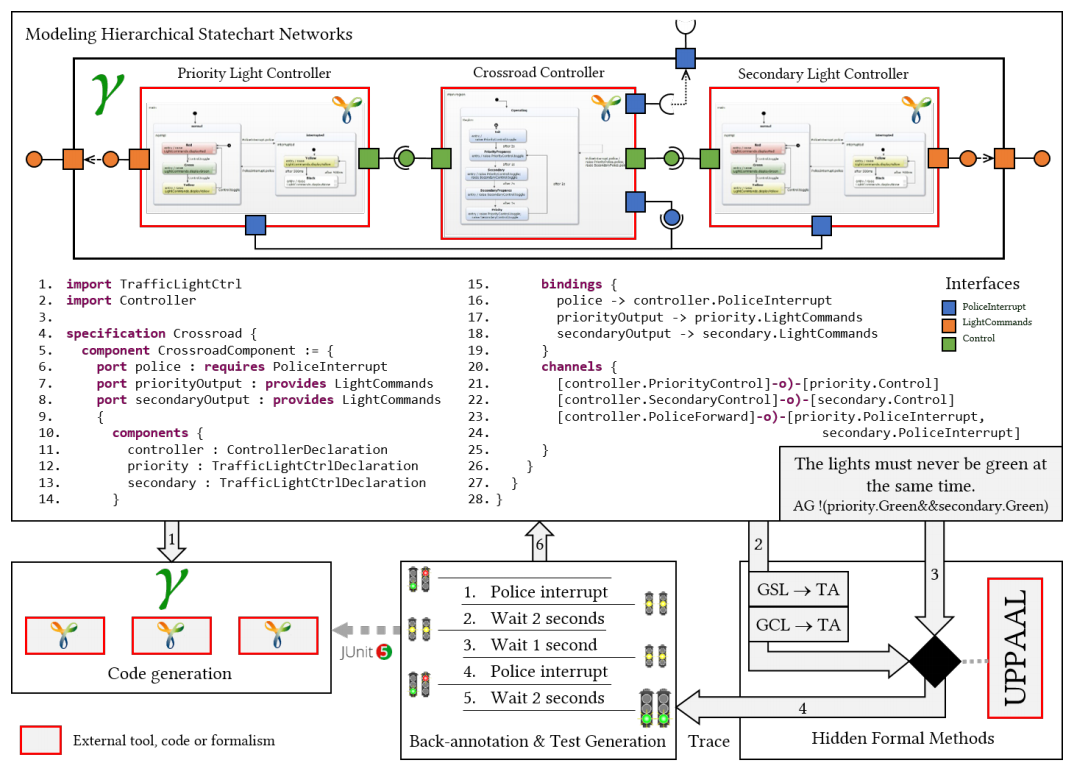
\includegraphics[width=140mm, keepaspectratio]{figures/preliminaries/gamma.png}
	%TODO Forras megjeloles!
	\caption[]{A Gamma Statechart Composition Framework\footnotemark}
	\label{fig:gamma}
\end{figure}
\newpage
A Gamma nagy erőssége, hogy állapotgép kompozíciókat is lehet modellezni benne. A komponenseket végrehajtás szempontjából háromféle szemantika van megkülönböztetve.

\paragraph{Szinkron komponensek} melyek egy lépésen belül fogadnak eseményeket ezekre lépnek és elküldik az eseményeket, ezek viszont a következő iterációban fognak fogadásra kerülni a hozzájuk kapcsolódó komponensekben.

\paragraph{Kaszkád komponensek (Cascade Component)} ezek hasonlóan működnek, mint a szinkron komponensek, viszont ebben az esetben a kiküldött üzenetek ugyan abban az iterációban kerülnek fogadásra. Ebből kifolyólag az üzenet áramlásnak aciklikusnak kell lennie, hiszen a feldolgozást végtelen ciklusba kerülne.

\paragraph{Aszinkron komponensek} Az események feldolgozása aszinkron módon, üzenet sorok kiolvasásával történik. Állapottérkép definíciók alapból szinkron szemantikával bírnak, így ahhoz hogy asszinkron szemantikával ruházzuk fel őket be kell csomagolni őket egy \emph{Wrapperbe}. Ez definiálja számukra az üzenet sort is.


\subsection{MagicDraw - Gamma transzformáció}

A MagicDraw beépülő modul fő célja SysML állapottérképek formális verifikációja. A Gamma képes állapotgépek ellenőrzésére ezek viszont a Gamma saját nyelvén kellenek, hogy legyenek definiálva. Modell transzformációk segítségével azonban lehetőségünk nyílik Gamma modellek származtatására SysML modellekből és ezáltal ellenőrizni őket.

Ez a származtatás vagy modell transzformáció képezi az ötlet alapját (\refstruc{fig:preliminaries-md-g}). A kihívás pedig az két nyelv közötti szemantikai különbségek feloldása illetve az elemek megfelelő egymáshoz rendelésének megtervezése és végrehajtása.

\begin{figure}[!ht]
	\centering
	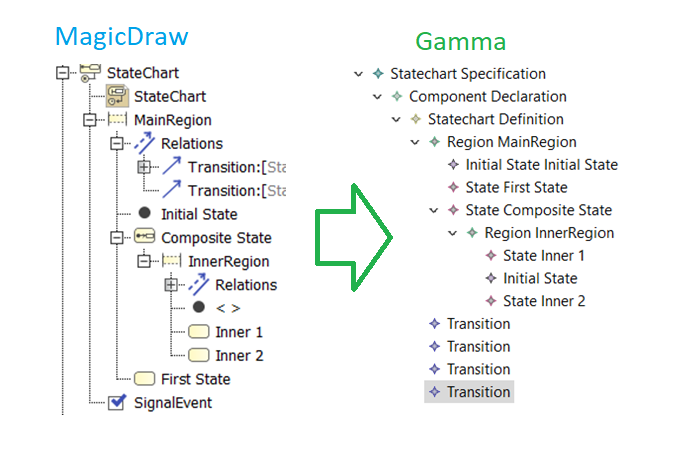
\includegraphics[width=150mm, keepaspectratio]{figures/preliminaries/md-g.png}
	\caption{Példa: egy modell transzformációra MagicDrawról Gammára}
	\label{fig:preliminaries-md-g}
\end{figure}

\subsection{Verifikáció menete}

A verifikáció elvégzése a MagicDraw beépülő modul szemszögéből négy lépésből áll: 
\begin{itemize}
	\item MagicDraw modellek Gammává transzformálása
	\item Gamma modellek \uppaal modellé transzformálása (ezt a Gamma keretrendszer végzi el)
	\item tulajdonságok ellenőrzése UPPAAL segítségével
	\item Eredmény megjelenítése
\end{itemize}
Ezt a folyamatot \refstruc{fig:preliminaries-verif} szemlélteti. A Gamma által elvégzett lépéseket a zöld "Gammák" jelölik a modellben. Az ábrán a verifikációt a "Módosított Query Generátor" kezdeményezi, mely szintén a "Gamma" jelölést kapta. Ennek oka, hogy a beépülő modul ezen verziójában az ellenőrizendő tulajdonságok megadása még nem volt kiforrott ezért egy a Gamma keretrendszerből átemelt megoldás segítségével lehetett ezeket megadni és a verifikációt kezdeményezni. 

\begin{figure}[!ht]
	\centering
	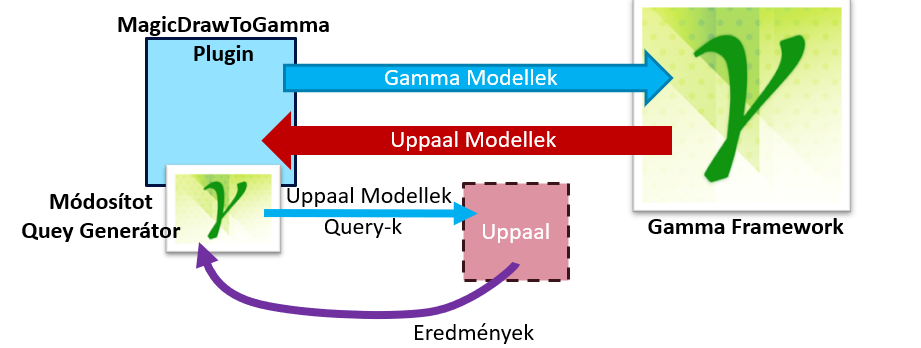
\includegraphics[width=150mm, keepaspectratio]{figures/preliminaries/concept.png}
	\caption{Verifikáció menete a pluginban}
	\label{fig:preliminaries-verif}
\end{figure}

\subsection{Őrfeltételek, akciók}

SysML nem definiál akció nyelvet őrfeltételek és akciók végrehajtásához. Míg akciókat tudunk modellezni bármilyen viselkedést leíró modell segítségével, addig az őrfeltételeket jellemzően valamilyen szöveges nyelvtannal szokás megadni.

Ahhoz, hogy a modell ellenőrzést végre lehessen hajtani ezeknek a Gamma számára érthető kifejezéseknek kell lenniük. A pluginnak ez a verziójában ezért minden őrfeltételt és akciót a Gamma által biztosított nyelvtan segítségével kellett megírni. Ez abból a szempontból nem szerencsés, hogy ez nem egy olyan elterjedt nyelv, mint például a javascript amit a MagicDraw felkínál, továbbá nem áll még rendelkezésre olyan interpreter a MagicDraw-ban ami lehetővé tenné ezek futtatását ami elengedhetetlen többek között a modellek szimulációjához.


\section{Xtext}

Az Xtext egy keretrendszer amivel programozási nyelveket és egyéb szakterület specifikus nyelveket lehet készíteni, melyek szöveges formában manifesztálódnak. Ezeket valamilyen már meglévő modellezési nyelv egy konkrét szintaxisaként érdemes készíteni. Ez azt jelenti, hogy egy szövegesen megadott leírás elemeket és ezek kapcsolatait írja egy metamodellnek megfelelően.

Az Xtext nyelvtanok készítéséhez egy erős nyelvtan leíró nyelvet kínál. Az ezzel leírt nyelvtanhoz pedig teljes infrastruktúrát generál mint: parser, linker, típus ellenőrző, fordító. Ezen felül Eclipses környezetben a szerkesztéshez kapunk szintaxis kiemelést, content assistot.

MagicDraw-ban is ki tudjuk használni az Xtextben rejlő lehetőségeket és akár saját kiértékelő motort is tudunk írni, az általunk létrehozott nyelvtanokhoz. Sajnos a MagicDraw beépített szerkesztőjében elesünk olyan hasznos felhasználói funkcióktól mint a content assist vagy a szintaxis kiemelés. Erre megoldást jelenthet az Xtext language szerver támogatásának a kihasználása a dolgozat azonban ennek a vizsgálatára nem tér ki.

Az Xtext használatára a dolgozat elkészítése során két helyen volt szükségem. Az egyik az őrfeltételek \emph{parse}olása, a másik pedig külön kérésre egy olyan export funkció integrálása ami XMI helyett a Gamma saját nyelvtanára sorosítva képes modelleket kimenteni.



